\chapter{Arhitektura i dizajn sustava}

    \begin{figure}[!h]
		\centering
		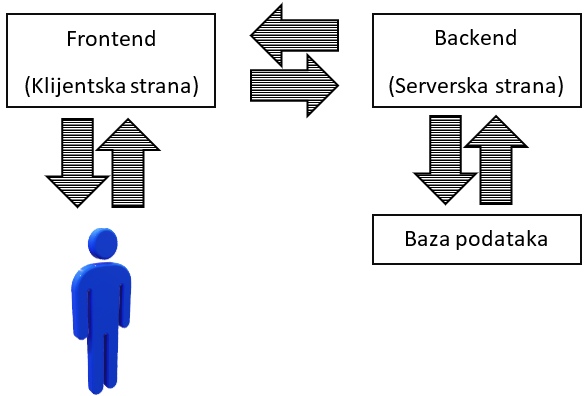
\includegraphics[width=13cm]{slike/arhitektura.PNG} 
		\caption{Arhitektura sustava}
		\label{fig:arhitektura}
	\end{figure}

	Korisnik aplikaciji pristupa putem web preglednika. Interakciju s aplikacijom ostvaruje preko korisničkog sučelja pomoću kojeg šalje zahtjeve web poslužitelju i prima odgovore.\\
Programski jezik pomoću kojeg je ostvaren backend web aplikacije je Java, a korišteni radni okvir je Spring Boot. Frontend aplikacije ostvaren je programskim jezikom JavaScript i bibliotekom React.js. Za razvojno okruženje odabran je Intellij IDEA. Spring Boot je radni okvir namijenjen stvaranju mikroservisa. Mikroservis je arhitektura koja omogućuje neovisan razvoj više različitih servisa od kojih svaki ima svoj proces.\\
Web aplikaciju čine tri osnovna dijela:
	\begin{itemize}
		\item 	\textbf{frontend}
		\item 	\textbf{backend}
		\item 	\textbf{baza podataka }		
	\end{itemize}
Frontend se sastoji od komponenata i logike. Istu komponentu je moguće koristiti za različite namjene (engl. reusability). React.js koristi virtualni DOM (engl. Document Object Model) čiji se sadržaj uspoređuje sa stvarnim DOM-om i na osnovu toga se provode promjene što za posljedicu ima poboljšanje performansi. Struktura ostvarena međusobnim povezivanjem različitih komponenti je stablo.\\
Backend se sastoji od: 
\begin{itemize}
		\item 	programskog sučelja za reprezentacijski prijenos stanja (REST API), odnosno Controller-a
		\item 	sloja poslovne logike (Service)
		\item 	sloja za pristup bazi podataka (Repository)		
	\end{itemize}
\textbf{Controller} izlaže funkcionalnost web aplikacije kao RESTful web usluge, tj. prima zahtjeve čiji su glavni dijelovi URI, metoda i HTTP zaglavlje, a korisniku šalje odgovor koji se sastoji od statusnog koda, tijela poruke i zaglavlja. U tijelu poruke se nalazi sadržaj kojeg korisnik konzumira nakon što je prikazan u web pregledniku. Komunikaciju sa slojem poslovne logike Controller ostvaruje pomoću umetanja ovisnosti (engl. dependency injection). Dependency injection je obrazac prema kojemu se u određeni objekt/funkciju umeće neki drugi objekt/funkcija na koji se prvobitno spomenuti objekt/funkcija oslanja.\\
\textbf{Service} omogućuje komunikaciju između slojeva Controller i Repository, zadužen je za provjeru ispravnosti podataka. Osim na sloju Service, provjera ispravnosti se obavlja na frontend-u i u bazi podataka. Komunikaciju sa slojem za pristup bazi podataka ostvaruje umetanjem ovisnosti.\\ 
\textbf{Repository} omogućuje komunikaciju s bazom podataka pomoću SQL-a. Objekti iz relacijske baze podataka pretvaraju se objekte programskog jezika Java korištenjem tehnike ORM.\\\\
		


		
		\textbf{\textit{dio 1. revizije}}\\

		\textit{ Potrebno je opisati stil arhitekture te identificirati: podsustave, preslikavanje na radnu platformu, spremišta podataka, mrežne protokole, globalni upravljački tok i sklopovsko-programske zahtjeve. Po točkama razraditi i popratiti odgovarajućim skicama:}
	\begin{itemize}
		\item 	\textit{izbor arhitekture temeljem principa oblikovanja pokazanih na predavanjima (objasniti zašto ste baš odabrali takvu arhitekturu)}
		\item 	\textit{organizaciju sustava s najviše razine apstrakcije (npr. klijent-poslužitelj, baza podataka, datotečni sustav, grafičko sučelje)}
		\item 	\textit{organizaciju aplikacije (npr. slojevi frontend i backend, MVC arhitektura) }		
	\end{itemize}

	
		

		

				
		\section{Baza podataka}
			
			\textbf{\textit{dio 1. revizije}}\\
			
		\textit{Potrebno je opisati koju vrstu i implementaciju baze podataka ste odabrali, glavne komponente od kojih se sastoji i slično.}
		
			\subsection{Opis tablica}
			

				\textit{Svaku tablicu je potrebno opisati po zadanom predlošku. Lijevo se nalazi točno ime varijable u bazi podataka, u sredini se nalazi tip podataka, a desno se nalazi opis varijable. Svjetlozelenom bojom označite primarni ključ. Svjetlo plavom označite strani ključ}
				
				\begin{longtblr}[
					label=none,
					entry=none
					]{
						width = \textwidth,
						colspec={|X[6,l]|X[6, l]|X[20, l]|}, 
						rowhead = 1,
					} %definicija širine tablice, širine stupaca, poravnanje i broja redaka naslova tablice
					\hline \textbf{korisnik - ime tablice} & \\ \hline[3pt]
					\SetCell{LightGreen}IDKorisnik & INT	&  	Lorem ipsum dolor sit amet, consectetur adipiscing elit, sed do eiusmod  	\\ \hline
					korisnickoIme	& VARCHAR &   	\\ \hline 
					email & VARCHAR &   \\ \hline 
					ime & VARCHAR	&  		\\ \hline 
					\SetCell{LightBlue} primjer	& VARCHAR &   	\\ \hline 
				\end{longtblr}
				
				
			
			\subsection{Dijagram baze podataka}
				\textit{ U ovom potpoglavlju potrebno je umetnuti dijagram baze podataka. Primarni i strani ključevi moraju biti označeni, a tablice povezane. Bazu podataka je potrebno normalizirati. Podsjetite se kolegija "Baze podataka".}
			
			\eject
			
			
		\section{Dijagram razreda}
		
			\textit{Potrebno je priložiti dijagram razreda s pripadajućim opisom. Zbog preglednosti je moguće dijagram razlomiti na više njih, ali moraju biti grupirani prema sličnim razinama apstrakcije i srodnim funkcionalnostima.}\\
			
			\textbf{\textit{dio 1. revizije}}\\
			
			\textit{Prilikom prve predaje projekta, potrebno je priložiti potpuno razrađen dijagram razreda vezan uz \textbf{generičku funkcionalnost} sustava. Ostale funkcionalnosti trebaju biti idejno razrađene u dijagramu sa sljedećim komponentama: nazivi razreda, nazivi metoda i vrste pristupa metodama (npr. javni, zaštićeni), nazivi atributa razreda, veze i odnosi između razreda.}\\
			
			\textbf{\textit{dio 2. revizije}}\\			
			
			\textit{Prilikom druge predaje projekta dijagram razreda i opisi moraju odgovarati stvarnom stanju implementacije}
			
			
			
			\eject
		
		\section{Dijagram stanja}
			
			
			\textbf{\textit{dio 2. revizije}}\\
			
			\textit{Potrebno je priložiti dijagram stanja i opisati ga. Dovoljan je jedan dijagram stanja koji prikazuje \textbf{značajan dio funkcionalnosti} sustava. Na primjer, stanja korisničkog sučelja i tijek korištenja neke ključne funkcionalnosti jesu značajan dio sustava, a registracija i prijava nisu. }
			
			
			\eject 
		
		\section{Dijagram aktivnosti}
			
			\textbf{\textit{dio 2. revizije}}\\
			
			 \textit{Potrebno je priložiti dijagram aktivnosti s pripadajućim opisom. Dijagram aktivnosti treba prikazivati značajan dio sustava.}
			
			\eject
		\section{Dijagram komponenti}
		
			\textbf{\textit{dio 2. revizije}}\\
		
			 \textit{Potrebno je priložiti dijagram komponenti s pripadajućim opisom. Dijagram komponenti treba prikazivati strukturu cijele aplikacije.}